\newpage
\section*{Appendix}
This section covers the original code.


\subsection*{Exercise 2 - Code for sampling, histograms and test}
\begin{python}
import numpy as np
import numpy.random as npr
import scipy.stats as stats
import matplotlib.pyplot as plt

# chi square test
def chisquared(expected, observed):
    nclass = len(expected)
    T = sum([(observed[i]-expected[i])**2/expected[i] for i\
             in range(nclass)])
    return T
def count(i, set):
    num = 0
    for j in set:
        if j == i:
            num += 1
    return num


### Geometric distribution
p = 1/3
N = 10000
GeoCrude = np.zeros(N)

k = np.arange(1,30,1)
pdfk = stats.geom.pmf(k,p)

c = (1-p)** 0 * p

# Do crude simulation
for i in range(N):
    U = npr.rand()
    X = np.int(np.log(U)/(np.log(1-p))) + 1
    GeoCrude[i] = X

plt.figure()
plt.hist(GeoCrude,density=True,ec='k',bins=range(0,25,1))
plt.plot(k,pdfk,'.-')
plt.title('Geometric with p = 1/3')
plt.show()

geoEx = [N * (1-p)**(i-1)*p for i in range(1, 25) ]
geoOb = [count(i, GeoCrude) for i in range(1, 25)]
print(chisquared(geoEx, geoOb))


### 6-point distribution
p = np.array([7/48,5/48,1/8,1/16,1/4,5/16])
N = 10000
F = np.cumsum(p)

SixCrude = np.zeros(N)


# Do crude simulation
for i in range(N):
    U = npr.rand()
    X = np.nonzero(U < F)[0][0] + 1
    SixCrude[i] = np.int(X)

plt.figure()
plt.hist(SixCrude,density=True,ec='k',bins=range(0,8,1))
plt.plot(np.arange(1,7),p,'.-')
plt.title('Crude pmf')
plt.show()

sixEx = (N * p).tolist()
crudeOb = [count(i, SixCrude) for i in range(1, 7)]
print(chisquared(sixEx, crudeOb))

# Reject sampling
c = np.max(p)
k = 6
ind = 0
SixReject = np.zeros(N)


while SixReject[N-1] == 0:
    I = 1 + np.int(k * npr.rand())
    if npr.rand() <= p[I-1]/c:
        SixReject[ind] = I
        ind += 1


plt.figure()
plt.hist(SixReject,density=True,ec='k',bins=range(0,8,1))
plt.plot(np.arange(1,7),p,'.-')
plt.title('Reject pmf')
plt.show()

rejectOb = [count(i, SixReject) for i in range(1, 7)]
print(chisquared(sixEx, rejectOb))


# Alias method
F = np.array([1,1/2,15/16,1,1/4,11/16])
L = np.array([1,4,1,4,3,3])
SixAlias = np.zeros(N)

for i in range(N):
    I = 1 + np.int(k * npr.rand())

    if npr.rand() <= F[I-1]:
        SixAlias[i] = I
    else:
        SixAlias[i] = L[I-1]

plt.figure()
plt.hist(SixAlias,density=True,ec='k',bins=range(0,8,1))
plt.plot(np.arange(1,7),p,'.-')
plt.title('Alias pmf')
plt.show()

aliasOb = [count(i, SixAlias) for i in range(1, 7)]
print(chisquared(sixEx, aliasOb))


\end{python}

\subsection*{Exercise 3 - Code}
\begin{python}
import numpy as np
import numpy.random as npr
import scipy.stats as stats
import matplotlib.pyplot as plt


N = 10000

### Exponential
varExp = np.zeros(N)
lam = 3

for i in range(N):
    varExp[i] = -np.log(npr.rand())/lam
# Get PDF

x = np.arange(0,2,0.01)
pdf = stats.expon.pdf(x,scale=1/lam)


plt.figure()
plt.hist(varExp,density=True,ec='k',bins=100)
plt.plot(x,pdf,'-')
plt.title('Exponential with lambda = 3')
plt.show()


### Normal distribution using Box-Mueller

N = 10000
Rsq = 2
V1 = 0
V2 = 0

varNorm = np.zeros(N)

for i in range(N):

    while Rsq > 1:
        V1 = -1 + 2*npr.rand()
        V2 = -1 + 2*npr.rand()
        Rsq = V1 ** 2 + V2 ** 2

    cos = V1 /np.sqrt(Rsq)
    sin = V2 /np.sqrt(Rsq)

    U = npr.rand()
    Z1 = np.sqrt(-2*np.log(U))*cos
    Z2 = np.sqrt(-2*np.log(U))*sin


    varNorm[i] = Z1
    Rsq = 2

x = np.arange(-4,4,0.01)
pdf = stats.norm.pdf(x,scale=1)


plt.figure()
plt.hist(varNorm,density=True,ec='k',bins=15)
plt.plot(x,pdf,'-')
plt.title('Standard normal box mueller')
plt.show()


#### Pareto


def pdfpar(x,k):
    return (x+1) ** (-k) * k / (x + 1)

# k = 2.05
beta = 1
k = 2.05
varPar = np.zeros(N)


x = np.arange(0,4,0.001)
pdf = pdfpar(x,k)


for i in range(N):
    U = npr.rand()
    varPar[i] = beta * ( U**(-1/k) - 1)

plt.figure()
plt.hist(varPar,density=True,ec='k',bins=100)
plt.plot(x,pdf,'-')
plt.title('Pareto k = 2.05')
plt.show()

p1 = varPar



# k = 2.5
beta = 1
k = 2.5
varPar = np.zeros(N)

for i in range(N):
    U = npr.rand()
    varPar[i] = beta * ( U**(-1/k) - 1)



x = np.arange(0,4,0.001)
pdf = pdfpar(x,k)

plt.figure()
plt.hist(varPar,density=True,ec='k',bins=100)
plt.plot(x,pdf,'-')
plt.title('Pareto k = 2.5')
plt.show()

p2 = varPar


# k = 3.0
beta = 1
k = 3.0
varPar = np.zeros(N)

for i in range(N):
    U = npr.rand()
    varPar[i] = beta * ( U**(-1/k) - 1)

x = np.arange(0,4,0.001)
pdf = pdfpar(x,k)

plt.figure()
plt.hist(varPar,density=True,ec='k',bins=100)
plt.plot(x,pdf,'-')
plt.title('Pareto k = 3.0')
plt.show()

p3 = varPar


# k = 4.0
beta = 1
k = 4.0
varPar = np.zeros(N)

for i in range(N):
    U = npr.rand()
    varPar[i] = beta * ( U**(-1/k) - 1)


x = np.arange(0,4,0.001)
pdf = pdfpar(x,k)
plt.figure()
plt.hist(varPar,density=True,ec='k',bins=100)
plt.title('Pareto k = 4.0')
plt.plot(x,pdf,'-')
plt.show()

p4 = varPar



#### Pareto with support beta > 1 k = 2.05

def pdfpar2(x,k):
    return (1/x) ** (k) * k / (x)

k = 2.05
beta = 1
varPar = np.zeros(N)

x = np.arange(1,4,0.001)
pdf = pdfpar2(x,k)


for i in range(N):
    U = npr.rand()
    varPar[i] = beta * ( U**(-1/k))

plt.figure()
plt.hist(varPar,density=True,ec='k',bins=1000)
plt.plot(x,pdf,'-')
plt.title('Pareto k = 2.05 and support beta > 1 ')
plt.show()

print(np.mean(varPar))
print(np.var(varPar))

p5 = varPar



# pareto with k =4.05 and support beta > 1
k = 4.0
beta = 1
varPar = np.zeros(N)

x = np.arange(1,4,0.001)
pdf = pdfpar2(x,k)


for i in range(N):
    U = npr.rand()
    varPar[i] = beta * ( U**(-1/k))

plt.figure()
plt.hist(varPar,density=True,ec='k',bins=100)
plt.plot(x,pdf,'-')
plt.title('Pareto k = 4.00 and support beta > 1 ')
plt.show()

print(np.mean(varPar))
print(np.var(varPar))

p6 = varPar



### Normal distribution simulated 100 times CI

nobs = 100
means = np.zeros(nobs)
variances = np.zeros(nobs)
Rsq = 2
V1 = 0
V2 = 0

for i in range(nobs):
    normvar = np.zeros(10)
    for j in range(10):
        while Rsq > 1:
            V1 = -1 + 2 * npr.rand()
            V2 = -1 + 2 * npr.rand()
            Rsq = V1 ** 2 + V2 ** 2

        cos = V1 / np.sqrt(Rsq)
        sin = V2 / np.sqrt(Rsq)

        U = npr.rand()
        Z1 = np.sqrt(-2 * np.log(U)) * cos
        Z2 = np.sqrt(-2 * np.log(U)) * sin
        normvar[j] = Z1
        Rsq = 2


    means[i] = np.mean(normvar)
    variances[i] = np.var(normvar)

CImeans = np.quantile(means,[0.025,0.975])
CIvariances = np.quantile(variances,[0.025,0.975])


###### KS test

# normal
normtest = stats.kstest(varNorm,'norm')
exptest = stats.kstest(varExp,'expon',args=(1/3))


partest1 = stats.kstest(p1,'lomax',args=(2.05,0))
partest2 = stats.kstest(p2,'lomax',args=(2.5,0))
partest3 = stats.kstest(p3,'lomax',args=(3.0,0))
partest4 = stats.kstest(p4,'lomax',args=(4.0,0))


partest5 = stats.kstest(p5,'pareto',args=(2.05,0))
partest6 = stats.kstest(p6,'pareto',args=(4.00,0))
\end{python}


\subsection*{Exercise 4 - Code}
\begin{python}
import numpy as np
import scipy.stats as stats
import numpy.random as npr
import matplotlib.pyplot as plt


### Exercise 4

# Number 1 - simple case both exponenial
def simple(n,muST,mu,Nsamples):
    Sn = np.zeros(n)
    T = 0
    reject = 0

    for i in range(Nsamples):
        X = npr.exponential(mu)
        T = T + X
        if (T >= np.min(Sn)):
            ind = np.argmin(Sn)
            Y = npr.exponential(muST)
            Sn[ind] = Y + T
        else:
            reject += 1

    return reject

def erlang(n,muST,mu,Nsamples):
    Sn = np.zeros(n)
    T = 0
    reject = 0

    for i in range(Nsamples):
        X = stats.erlang.rvs(1, loc=0, scale=1, size=1)
        T = T + X
        if (T >= np.min(Sn)):
            ind = np.argmin(Sn)
            Y = npr.exponential(muST)
            Sn[ind] = Y + T
        else:
            reject += 1

    return reject

def pareto1(n,muST,mu,Nsamples):
    Sn = np.zeros(n)
    T = 0
    reject = 0

    for i in range(Nsamples):
        X = npr.exponential(mu)
        T = T + X
        if (T >= np.min(Sn)):
            ind = np.argmin(Sn)
            Y = stats.pareto.rvs(2.05, scale=4.1, size = 1)
            Sn[ind] = Y + T
        else:
            reject += 1

    return reject

def const(n,muST,mu,Nsamples):
    Sn = np.zeros(n)
    T = 0
    reject = 0

    for i in range(Nsamples):
        X = npr.exponential(mu)
        T = T + X
        if (T >= np.min(Sn)):
            ind = np.argmin(Sn)
            Y =  8
            Sn[ind] = Y + T
        else:
            reject += 1

    return reject


def Cint(theta,alpha):
    mu = np.mean(theta)
    df = len(theta)-1
    S = np.std(theta)
    n = len(theta)
    t = stats.t.ppf(alpha/2,df=df)
    CI = np.mean(theta) + S/np.sqrt(n) * t * np.array([1,-1])

    return CI


rejectA = np.zeros(10)
for j in range(10):
    rejectA[j] = pareto1(10,8,1,10000)

CIA = Cint(rejectA,0.05)
print(CIA,sum(rejectA)/10)




\end{python}

\subsection*{Exercise 6 - Code}
Individual code are appended for this exercise and the following exercise since these two are more complicated. 

\textbf{Sen's code:}
\begin{python}
# Ex. 6 MH algorithm

import math
from random import random

def gi(i, A = 8):
    return (A**i)/(math.factorial(i))
giSum = sum([gi(i) for i in range(11)]) 

# chi square test
def chisquared(setA, setB):
    nclass = len(setA)
    T = sum([(setB[i]-setA[i])**2/setA[i] for i in range(nclass)])
    return T

def count(i, set):
    num = 0
    for j in set:
        if j == i:
            num += 1
    return num

sample = 10000
burn_in = 5000

X = [0] * (sample + burn_in)

incb = 5 #incumbent

for i in range(sample + burn_in):
    
    if random() <= 0.5:
        delta = 1 # deltaX
    else:
        delta = -1
    
    Y = incb + delta
    if Y == -1:
        Y = 10
    if Y == 11:
        Y = 0
        
    if gi(Y)>= gi(incb):
        incb = Y
    else:
        if random() <= gi(Y)/gi(incb):
            incb = Y
    X[i] = incb

result = X[burn_in: burn_in + sample] # obtained samples

# chi squared test
expected = [gi(i)*sample/giSum for i in range(11)]
observed = [count(i, result) for i in range(11)]
T = chisquared(expected, observed)

print(T)

\end{python}
Output: T = 12.2, then p = 0.2023.

\begin{python}
# direct MH for two-dimensional problem

import math
from random import random
import matplotlib.pyplot as plt

def gi(i, j, A = 4):
    return (A**i)/(math.factorial(i)) * (A**j)/(math.factorial(j))
gi_sum = 0
for i in range(10):
    for j in range(10):
        gi_sum += gi(i, j)


# directly MH
sample = 150000
burn_in = 1000

X = [0] * (sample + burn_in)  # sample
Y = [0] * (sample + burn_in)

incbX = 2  # initial value
incbY = 2

for ind in range(sample + burn_in):
    randX = random()
    randY = random()
    deltaX = int(randX*3) -1
    deltaY = int(randY*3) -1
    
    incbX1 = incbX + deltaX
    incbY1 = incbY + deltaY
    
    if incbX == 5 and incbY == 5 and (incbX1 + incbY1) > 10:
        incbX1 = 0
        incbY1 = 0
    
    if incbX == 0 and incbY == 0:
        if incbX1 + incbY1 < 0:
            incbX1 = 5
            incbY1 = 5
        elif incbX1 + incbY1 == 0:
            incbX1 = 0
            incbY1 = 0
    
    if incbX1 + incbY1 > 10:
        incbX1 = incbY
        incbY1 = incbX

    if incbX1 < 0 or incbY1 < 0:
        incbX1 = incbY
        incbY1 = incbX
        
    if gi(incbX1, incbY1) >= gi(incbX, incbY):
        incbX = incbX1
        incbY = incbY1
    
    else:
        if random() <= gi(incbX1, incbY1)/gi(incbX, incbY):
            incbX = incbX1
            incbY = incbY1
    
    X[ind] = incbX
    Y[ind] = incbY

'''
true1 = []
true2 = []
for i in range(11):
    for j in range(11-i):
        num_sample = int(gi(i, j) / gi_sum * sample)
        true1 += ([i]*num_sample)
        true2 += ([j]*num_sample)
        
plt.hist2d(true1, true2, bins = 10)
'''
plt.hist2d(X, Y, bins = 10)
plt.xlabel('i')
plt.ylabel('j')
cbar = plt.colorbar()
cbar.ax.set_ylabel('Counts')
plt.show()
\end{python}

For the coordinate-wise case, only slight change is made to the aforementioned code, which is shown in the follows to limit that deltaX and deltaY cannot be non-zero at the same time.
\begin{python}
    if random() <= 0.5:
        deltaX = 0
    else:
        deltaY = 0
\end{python}

\begin{python}
# gibbs sampling

import numpy.random as npr
import matplotlib.pyplot as plt
import math
from random import random

def gi(i, A = 4):
    return (A**i)/(math.factorial(i))

# compute the conditional probability
def p_con(i, j): # probability of j under i
    p = gi(i) * gi(j) / sum([gi(i)*gi(k) for k in range(11-i)])
    return p
    
sample = 50000
burn_in = 1000

incbx = 2
incby = 2

X = [0] * (sample + burn_in) 
Y = [0] * (sample + burn_in)
for ind in range(sample + burn_in):
    I = npr.randint(2)
    
    if I == 0:      
        cdf = [sum([p_con(incby,t) for t in range(i+1)])\
               for i in range(11)]
        U = random()
        for i in range(11):
            if cdf[i] >= U:
                incbx1 = i
                break
        incby1 = incby
    else:
        cdf = [sum([p_con(incbx,t) for t in range(i+1)])\
               for i in range(11)]
        U = random()
        for i in range(11):
            if cdf[i] > U:
                incby1 = i
                break
        incbx1 = incbx


    if incbx1 + incby1 <= 10:
        incbx, incby = incbx1, incby1
    X[ind] = incbx
    Y[ind] = incby
 
plt.hist2d(X, Y, bins = 10)
plt.xlabel('i')
plt.ylabel('j')
cbar = plt.colorbar()
cbar.ax.set_ylabel('Counts')
plt.show()       
\end{python}
\textbf{Output:}
\begin{figure}[H]
\centering
\begin{subfigure}{.5\textwidth}
  \centering
  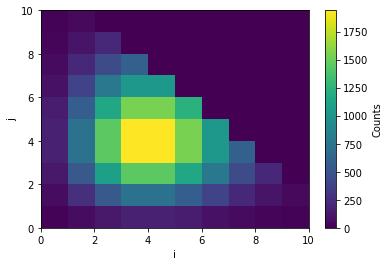
\includegraphics[width=.8\linewidth]{figures/truesen.png}
  \caption{True}
\end{subfigure}%
\begin{subfigure}{.5\textwidth}
  \centering
  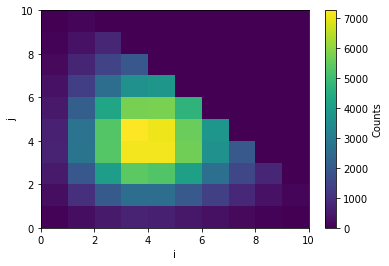
\includegraphics[width=.8\linewidth]{figures/simplesen.png}
  \caption{Simple MH}
\end{subfigure}\\
\begin{subfigure}{.5\textwidth}
  \centering
  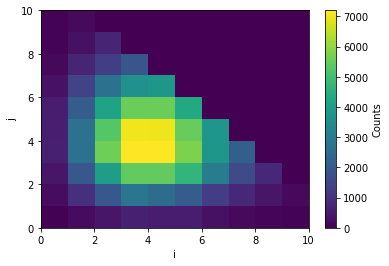
\includegraphics[width=.8\linewidth]{figures/coordinatesen.png}
  \caption{Coordinate}
\end{subfigure}%
\begin{subfigure}{.5\textwidth}
  \centering
  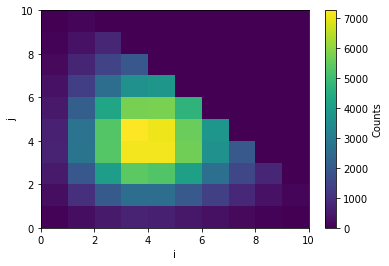
\includegraphics[width=.8\linewidth]{figures/simplesen.png}
  \caption{Gibbs}
\end{subfigure}
\end{figure}

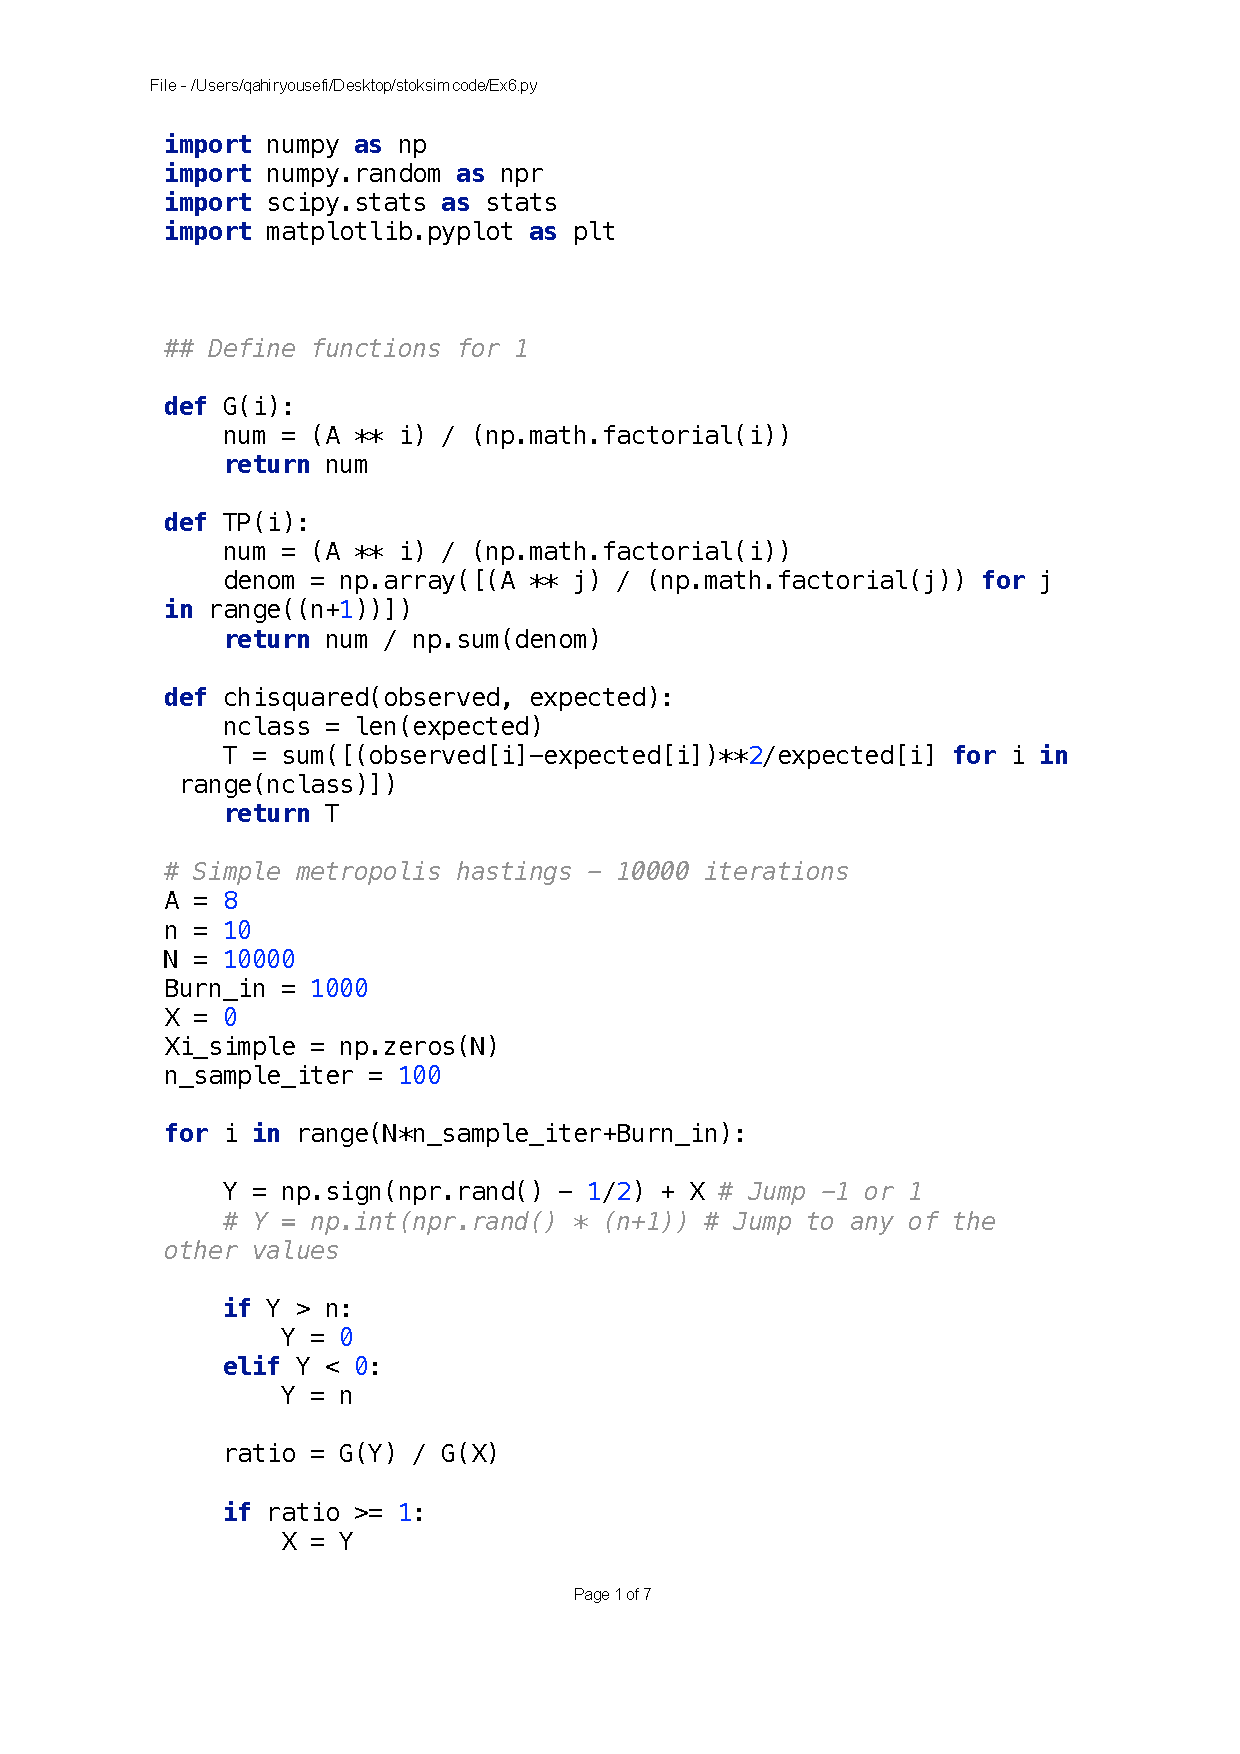
\includepdf[pages=-]{ex6.pdf}

\subsection*{Exercise 7 - code}
\textbf{Sen's code}
\begin{python}
# debug process
import math
import matplotlib.pyplot as plt
import numpy.random as npr
from random import random

def distance(j, k):
    Nstat = 12
    x = [0] * Nstat
    y = [0] * Nstat
    
    for i in range(Nstat):  # define the space
        x[i] = math.cos(2*math.pi/Nstat*i)*10
        y[i] = math.sin(2*math.pi/Nstat*i)*10
    return (math.sqrt( (x[k] - x[j])**2 + (y[k] - y[j])**2 ))

def cost(set1):
    cost1 = 0
    for i in range(len(set1)-1):
        cost1 += distance(set1[i], set1[i+1])
    cost1 += distance(set1[len(set1)-1], set1[0])
    return cost1
 
def swap(set1):
    length = len(set1)
    i, j = npr.randint(length, size = 2)
    set1[i], set1[j] = set1[j], set1[i]
    return set1

pi = math.pi

Nstat = 12
sample = 10000
x = [0] * Nstat
y = [0] * Nstat

for i in range(Nstat):  # define the space
    x[i] = math.cos(2*pi/Nstat*i)*10
    y[i] = math.sin(2*pi/Nstat*i)*10

route1 = npr.permutation(Nstat).tolist()
route_opt = route1[:]
cost_opt = cost(route_opt)

for ind in range(sample):
    T = 1/math.sqrt(1+ind)
    route0 = route1[:]
    route2 = swap(route0)
    if cost(route2) <= cost(route1):
        route1 = route2[:]
    else:
        if random() <= math.exp( ( cost(route1)-cost(route2) ) /T ):
            route1 = route2[:] 
    
    if cost(route1) < cost(route_opt):
        route_opt = route1[:]
        cost_opt = cost(route_opt)
    
    X = [x[i] for i in route_opt]
    X.append(X[0])
    Y = [y[i] for i in route_opt]
    Y.append(Y[0])
plt.plot(X, Y, '.-')
plt.show()
print(cost_opt)
\end{python}
\begin{python}
# TSP for given matrix
import math
import numpy.random as npr
from random import random
import pandas as pd
import matplotlib.pyplot as plt


def swap(set1):
    length = len(set1)
    i, j = npr.randint(length, size = 2)
    set1[i], set1[j] = set1[j], set1[i]
    return set1

def cost(set):
    cost1 = pd.read_excel (r'G:\dtumaster\stochasticSimulation\
                           \code\cost.xlsx', sheet_name='Sheet1')
    cost2 = 0
    for i in range(len(set)-1):
        cost2 += cost1.iloc[set[i],set[i+1]]
    cost2 += cost1.iloc[set[len(set)-1], set[0]]
    return cost2


Nstat = 20
sample = 5000


route1 = npr.permutation(Nstat).tolist()
route_opt = route1[:]
cost_opt = cost(route_opt)
opt_set = []

for ind in range(sample):
    T = 1/math.sqrt(1+ind)
    route0 = route1[:]
    route2 = swap(route0)
    if cost(route2) <= cost(route1):
        route1 = route2[:]
    else:
        if random() <= math.exp( ( cost(route1)-cost(route2) ) /T ):
            route1 = route2[:] 
    
    if cost(route1) < cost(route_opt):
        route_opt = route1[:]
        cost_opt = cost(route_opt)
    print(ind, cost_opt)
    opt_set.append(cost_opt)
    
print(route_opt)
print(cost_opt)

plt.plot(range(sample), opt_set)
plt.xlabel('iteration')
plt.ylabel('optimized cost')
plt.show()

\end{python}


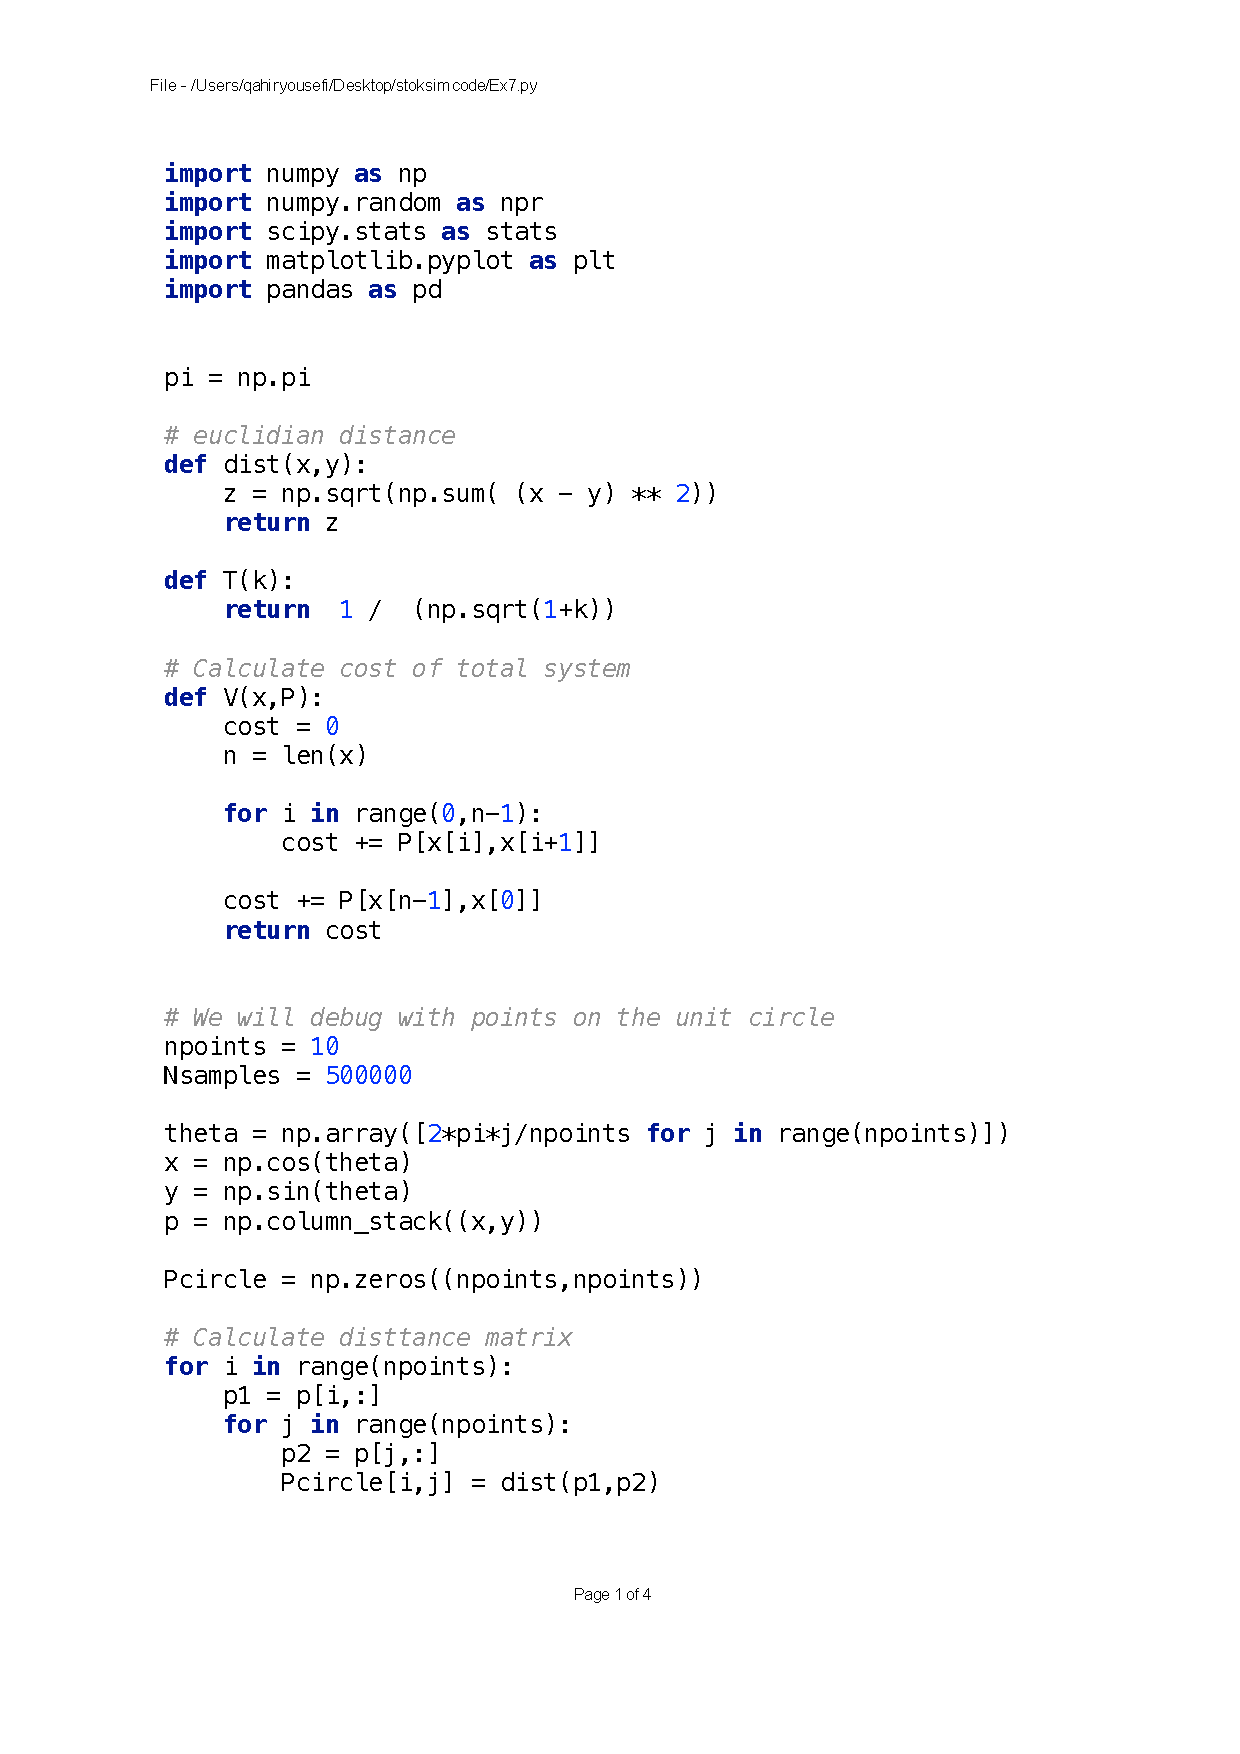
\includepdf[pages=-]{ex7.pdf}

\subsection*{Exercise 8 - Code}
\begin{python}
import numpy as np
import math
import scipy.stats as stats 
import statistics as stt
from Ex4 import Cint

'''
def bootstrap(X, test): # test is the number of tests
    sample = len(X)
    meanSet = [0] * test
    for i in range(test):
        sampleSet = [0] * sample
        for j in range(sample):
            sampleSet[j] = X[int(10 * np.random.random())]
        meanSet[i] = sum(sampleSet) / sample
    
    return meanSet, sum(meanSet)/test, np.var(meanSet)
        
    
X = [56, 101, 78, 67, 93, 87, 64, 72, 80, 69]
test = 8

mean = np.mean(X)

set_boot, mu, var = bootstrap(X, test)
a = - 5
b = 5

p = stats.norm.cdf((mean - a - mu)/math.sqrt(var))\
 - stats.norm.cdf((mean - b - mu)/math.sqrt(var))
'''

def bootstrap1(X, test): # test is the number of tests
    median_1 = stt.median(X)
    sample = len(X)
    medianSet = [0] * test
    for i in range(test):
        sampleSet = [0] * sample
        for j in range(sample):
            sampleSet[j] = X[int(10 * np.random.random())]
        medianSet[i] = stt.median(sampleSet)
    
    return median_1, medianSet, np.mean(medianSet), np.var(medianSet)

# simulate a Pareto distribution
N = 200
pareto = stats.pareto.rvs(b = 1.05, scale = 1, size = N)
meanp = np.mean(pareto)
medianp = np.median(pareto)
medianb, sett, mean_medianb, median_var = bootstrap1(pareto, 100)

def bootstrap(X, test): # test is the number of tests
    sample = len(X)
    meanSet = [0] * test
    for i in range(test):
        sampleSet = [0] * sample
        for j in range(sample):
            sampleSet[j] = X[int(10 * np.random.random())]
        meanSet[i] = sum(sampleSet) / sample
    
    return meanSet, sum(meanSet)/test, np.var(meanSet)
a, b, c = bootstrap(pareto, 100)

print(Cint(a, 0.05))

print(Cint(sett, 0.05))


\end{python}
